\bghdr{images/fond-infobr}

%\subsection{Configuration de ton navigateur \emph{Web}}
%\label{browser}
%Si ce n'est pas indiqué ici penses à configurer le proxy en suivant les instructions sur l'InfoBR en ligne (\urllink{https://portail.polytechnique.edu/dsi/acces-internet/proxy-eleves}
%\paragraph{Firefox}
%\flimage{images/firefox-logo}{0.07}{l}

%Lance \app{Mozilla Firefox}, et va dans le menu \menu{Outils},
%\menu{Options...} (ou \menu{Édition}, \menu{Prèfèrences...} sous Linux). Là , sélectionne la rubrique \menu{Avancé}, onglet \menu{Réseau}, et clique sur
%\menu{Paramètres}. La case à  cocher est alors \menu{Adresse de configuration automatique du proxy},
%et l'adresse à  indiquer est~: \urllink{http://config/proxy.pac}.

%Il te faut accepter le certificat SSL du BR. Cela consiste à indiquer que tu fais confiance au BR pour authentifier les sites des binets.\\
%Il suffit se se rendre sur \urllink{http://config/ca-br.crt} et de cocher toutes les cases.\\
%
%\noindent
%  \begin{figure*}[!h]
%    \begin{center}
%      %\subfloat[Configuration du serveur mandataire]{
%      %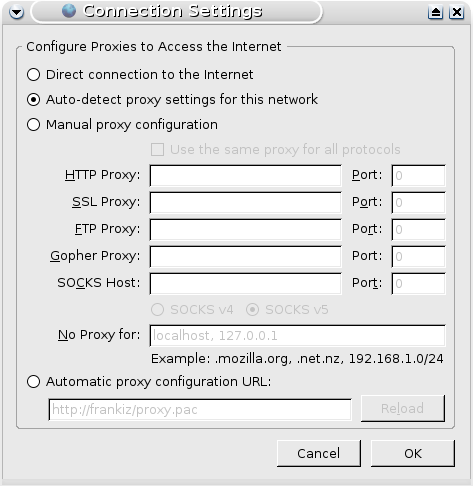
\includegraphics[width=0.48\textwidth]{images/nux_proxy_firefox}}
%      %\hspace{\stretch{1}}
%      \subfloat[Acceptation du certificat BR]{
%         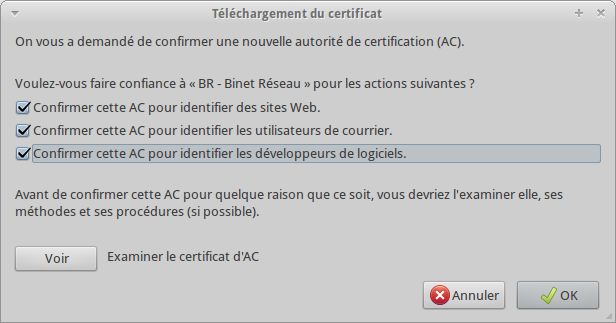
\includegraphics[width=0.48 \textwidth]{images/ca-br-ff}}
%           \caption{Configuration de Firefox}
%    \end{center}
%  \end{figure*}
%\imagepos{images/nux_proxy_firefox}{0.65}{Configuration du serveur mandataire sous Firefox}{ht}\\
%\imagepos{images/ca-br}{1}{Acceptation du certificat BR}{ht}
%
% Pour le RTFIBRp11 pour un saut de page si nécéssaire ce qui n'était pas le cas en 2008

%\noindent\rule{.4\textwidth}{.4pt}

%\vfill %\pagebreak


%\paragraph{Google Chrome}
%\flimage{images/google-chrome-logo}{0.07}{l}

%Pour \app{Google Chrome}, la configuration du serveur mandataire se règle automatique sur celle du système. Tu n'es donc pas obligè de règler le \emph{proxy} toi-même. Cependant, pour le faire manuellement, clique sur la
%clef à molette en haut à droite, choisis \menu{Options}, va dans l'onglet \menu{Paramètres avancès} (ou \menu{Under the Hood}), clique sur \menu{Modifier les paramètres du Proxy...} et règle comme ci-dessus.\\

%Pour accepter le certificat BR, il te faut d'abord le télécharger sur \urllink{http://config/ca-br.crt}.
%Puis, dans Chrome, rends-toi dans \menu{Préferences}, \menu{Options avancées}, \menu{Gérer les certificats},
%\menu{Autorités} et clique sur \menu{Importer}. Il suffit alors de sélectionner l'emplacement où tu avais stocké le certificat et de cocher toutes les cases.
%\imagepos{images/ca-br-chrome}{1}{Acceptation du certificat BR sous Google Chrome}{ht}

%\paragraph{Konqueror}
%\flimage{images/konqueror-logo}{0.07}{l}

%Sous \app{Konqueror}, cela se trouve dans le menu \menu{Configuration}, \menu{Configurer Konqueror},
%dans l'onglet \menu{Serveur mandataire}~; ensuite, choisis les même règlages que pour \app{Firefox} ci-dessus.
%Konqueror se configure de la même manière que \app{firefox} ci dessus.
%Attention~: si tu ne configures pas le serveur mandataire dans Konqueror,
%les logiciels KDE (\app{KGet}, \app{Adept},\dots) ne l'utiliseront pas~!


%%% pas besoin de configurer au niveau navigateur sur Mac OS
%\paragraph{Safari}
%\flimage{images/mac_safari_icone}{0.07}{l}

%\app{Safari}, le navigateur web d'Apple, est maintenant compatible avec la majorité des sites \emph{web}. Tu peux donc t'en servir au quotidien,
%en faisant appel à  \app{Firefox} pour les sites récalcitrants.

%% CE TRUC EST PAS A SA PLACE ICI.

 % \item \app{vlc}~: Un logiciel qui te permettra de recevoir la télévision directement dans ton casert, afin d'être vraiment sur d'avoir autre chose à  faire que travailler les veilles de pâles. Configuration page \pageref{TV}.



%%%%%%%%%%%%%%%%%%%%%%%%%%%%%%%%%%%%%%%%%%%%%%%%%%%%%%%%%%%%%%%%%%%%
%                            MAIL                                  %
%%%%%%%%%%%%%%%%%%%%%%%%%%%%%%%%%%%%%%%%%%%%%%%%%%%%%%%%%%%%%%%%%%%%

\subsection{Les mails}

La DSI met à ta disposition l'adresse \mail{prenom.nom@polytechnique.edu}.
Par défaut cette adresse redirige vers celle que tu as fournie à SCEI-Concours.
Tu peux changer cette redirection en allant sur \urllink{https://mail.polytechnique.fr/}.
Ne t'inquiète pas si ton navigateur affiche un avertissement quand tu te connectes, c'est juste que le certificat de la DSI n'est pas approuvé.
Commence par cliquer sur \emph{connexion} en haut à droite, le login est \mail{prenom.nom}.
Le mot de passe t'a été donné par la DSI lors de l'inkhôrpo.
Mais ce n'est pas grave si tu l'as perdu, tu peux en récupérer un nouveau en cliquant sur "Si vous avez perdu votre mot de passe...".
Le nouveau mot de passe te sera renvoyé sur ton adresse \mail{polytechnique.edu}, donc redirigé par défaut vers l'adresse que tu as donnée à SCEI.
Si tu ne peux plus accéder à cette adresse, il va falloir aller voir la DSI... Ils pourront changer tes redirections.

Si tu veux envoyer des mails avec ton adresse en \mail{polytechnique.edu}, la DSI a mis en place un nouveau webmail, auquel tu peux accéder en allant sur \urllink{webmail/}, ou depuis l'extérieur du plâtal \urllink{webmail.polytechnique.edu}.

%\subsection{Configuration de ton client \emph{mail}}
%
%La DSI met à  ta disposition une bo\^{i}te aux lettres électronique sur
%le serveur \server{poly}~; cette section t'explique comment
%configurer \app{Windows Mail}, \app{Kmail} et \app{Mac OS Mail} pour y avoir accès. Tu peux bien
%s\^{u}r utiliser \app{Thunderbird} si tu préfères, les données à  rentrer
%pour la configuration sont les mêmes~; quelques détails sont donnés
%dans le WikiX sur \fkz. De plus, tu trouveras des explications plus
%détaillées dans le manuel rédigé par la DSI.
%
%\paragraph{Outlook et Windows Mail}
%\flimage{images/outlook-logo}{0.07}{l}
%
%La procédure suivante fonctionne aussi avec \app{Windows Mail}.
%Lance \app{Outlook Express} et va dans le menu \menu{Outils},
%\menu{Comptes\ldots}. Clique sur le bouton \menu{Ajouter\ldots} en
%haut à  droite, puis sur \menu{Courrier\ldots}.
%
%Pour \app{Windows Mail} c'est sur compte de messagerie qu'il faut cliquer, avant de cliquer sur suivant.
%
%Remplis les écrans de configuration avec les données suivantes.
%\begin{description}
%  \item[Nom complet~: ] ton nom (\guillemotleft~Martin Durand~\guillemotright , par exemple)
%  \item[Adresse de messagerie~: ] de la forme \mail{prenom.nom@polytechnique.edu}
%  \item[Type de serveur de messagerie pour le courrier entrant~: ] \menu{POP3}
%  \item[Serveur de messagerie pour le courrier entrant~: ] \server{poly.polytechnique.fr}
%  \item[Serveur de messagerie pour le courrier sortant~: ] \server{poly.polytechnique.fr} ou \newline \server{ssl.polytechnique.org}
%  \item[Nom du compte~: ] ton identifiant \server{poly} (en gènèral c'est \texttt{prenom.nom}, si ça ne marche pas, va voir le bureau \emph{login} de la DSI.)
%  \item[Mot de passe~: ] ton mot de passe \server{poly}
%       vérifie bien que la case \menu{Mémoriser le mot de passe} est cochée.
%\end{description}
%
%Voilà , clique sur \menu{Continuer}, \menu{Terminer}.
%
%Tu te retrouves alors sur la fenêtre \menu{Comptes Internet}. Va sur
%l'onglet \menu{Courrier}, clique sur le compte que tu viens de créer
%puis sur \menu{Propriétés}. Clique sur l'onglet \menu{Avancé} et
%configure comme sur la capture~\ref{config:win:mail}~; en
%particulier, coche la seconde case \menu{Ce serveur nécessite une
%connexion sécurisée (SSL)}.
%
%Comme ça, tu peux désormais recevoir des \emph{mails} avec une liaison
%sécurisée vers \server{poly} pour que personne ne puisse les
%intercepter. Il est possible que tu aies à accepter manuellement le certificat utilisè par l'École pour que cela fonctionne correctement. Tu le trouveras sur \urllink{http://poly}. Une fois téléchargé, il suffit de l'importer.
%
%\imageref{images/win_config_mail_avance}{0.5}{Configuration avancée
%des serveurs \emph{mail}}{!h}{config:win:mail}
%
%
%
%\paragraph{Kmail}
%\flimage{images/kmail-logo}{0.07}{l}
%
%Pour \app{Kmail}, va dans \menu{Configuration}, \menu{Configurer Kmail}. Choisis la
%rubrique \menu{Comptes}. Commence par créer un nouveau compte dans
%l'onglet \menu{Réception des messages} en cliquant sur le bouton
%\menu{Ajouter\ldots} et choisis le type POP3.
%
%
%\noindent
%  \begin{figure*}[!h]
%    \begin{center}
%      \subfloat[Réception des messages]{
%      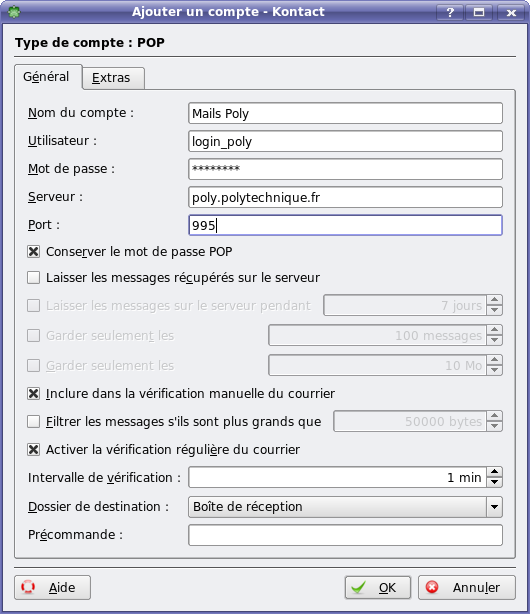
\includegraphics[width=0.48\textwidth]{images/nux_config_kmail_pop} }
%      \hspace{\stretch{1}}
%      \subfloat[Envoi des messages]{
% 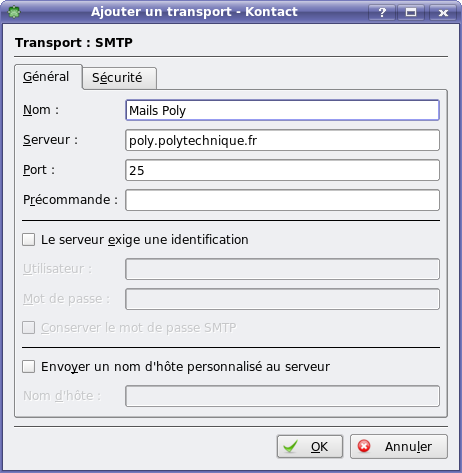
\includegraphics[width=0.48 \textwidth]{images/nux_config_kmail_smtp} }
% \caption{Configuration sous \app{Kmail}}
%    \end{center}
%  \end{figure*}
%
%
%Utilise les paramètres suivants pour configurer l'onglet \menu{Général}.
%\begin{description}
%  \item[Nom~: ] le nom du compte, par exemple~: Mails Poly
%  \item[Utilisateur~: ] l'identifiant \server{poly} que t'a fourni la DSI à  ton arrivée sur le plateau
%  \item[Mot de passe~: ] le mot de passe \server{poly}
%  \item[Serveur~: ] \server{poly.polytechnique.fr}
%  \item[Port~: ] 995
%\end{description}
%Ensuite, va dans l'onglet \menu{Extras} et coche la case
%\menu{Utiliser SSL pour sécuriser les téléchargements}.
%
%Maintenant, dans l'onglet \menu{Envoi des messages} clique sur le
%bouton \menu{Ajouter\ldots}. Utilise les paramètres suivants pour le
%configurer~:
%\begin{description}
%  \item[Nom] le même nom de compte que précédemment
%  \item[Serveur] \server{poly.polytechnique.fr} ou \server{ssl.polytechnique.org}
%  \item[Port] 25
%\end{description}
%Sinon, laisse toutes les cases décochées.
%
%%Tu peux aussi configurer l'accès à  \app{l'annuaire LDAP} de l'École, sorte de carnet d'adresses en ligne qui contient les adresses \emph{mail} de tout le monde sur le campus. Pour ce faire, commence par ouvrir \menu{Outils}, \menu{Carnet d'adresses}, puis va dans \menu{Configuration}, \menu{Configurer kAdressBook}, \menu{Consultation LDAP}. Clique ensuite sur \menu{Ajouter un hôte}, et configure comme suit: \\
%%\smallskip
%%\begin{minipage}[t]{0.48\textwidth}
%%\begin{description}
%%  \item[Hôte] \server{ldap.eleves.polytechnique.fr}
%%  \item[Port] 389
%%  \item[Version de LDAP] 3
%%\end{description}
%%\end{minipage}
%%\begin{minipage}[t]{0.48\textwidth}
%%\begin{description}
%%  \item[DN] \server{dc=polytechnique, dc=ldap, dc=eleves, dc=fr}
%%  \item[Sécurité] Non
%%  \item[Identification] Anonyme
%%\end{description}
%%\end{minipage} \\
%%Une fois revenu dans \menu{Configuration LDAP}, coche la case \server{ldap.eleves.polytechnique.fr}. Tu as maintenant accès à  l'annuaire LDAP lors de la
%%rédaction de messages, avec tout au plus un redémarrage de \app{Kmail}.
%%
%%\imagepos{images/nux_config_ldap}{0.55}{Configuration de l'annuaire LDAP sous Kmail}{pht}
%%\imagepos{images/nux_config_knode}{0.45}{Configuration de Knode}{ht}
%%
%%\noindent
%%  \begin{figure*}[!h]
%%    \begin{center}
%%      \subfloat[Configuration de l'annuaire LDAP sous Kmail]{
%%      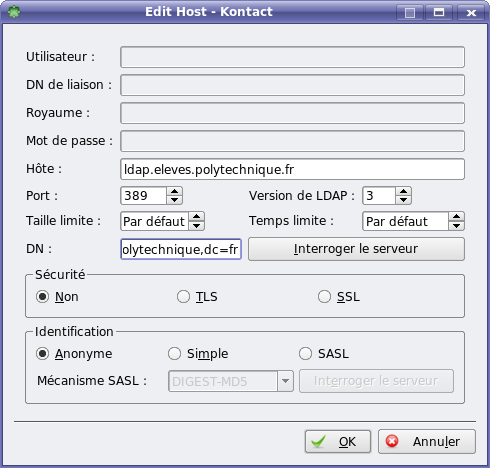
\includegraphics[width=0.48\textwidth]{images/nux_config_ldap}}
%%      \hspace{\stretch{1}}
%%      \subfloat[Configuration de Knode]{
%% 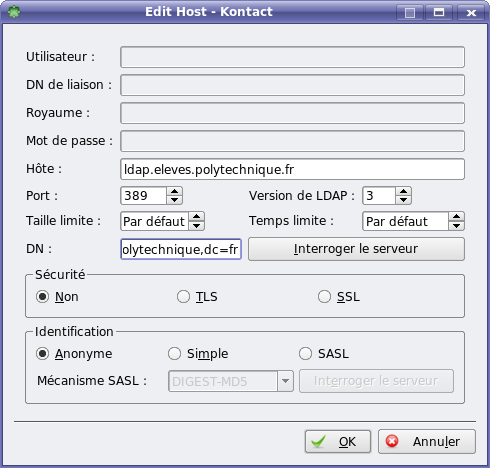
\includegraphics[width=0.48 \textwidth]{images/nux_config_ldap} }
%% \caption{Configurations LDAP et \emph{news}}
%%    \end{center}
%% \end{figure*}
%
%
%\paragraph{Mac OS Mail}
%
%\flimage{images/mac_mail_icone}{0.07}{l} \app{Mail}~: un client \emph{mail} offrant les fonctionnalités classiques d'un bon client~: recherche instantanée, filtre antispam, règles de tri automatique des \emph{mails}, regroupement des \emph{mails} correspondant à  une même discussion.
%
%Au premier lancement, \app{Mail} te demandera de remplir les informations concernant ton compte \emph{mail} sur \server{poly}, il suffit de le remplir avec les données suivantes~:
%\begin{description}
%  \item[Nom complet] ton nom~!
%  \item[Adresse électronique] de la forme \mail{prenom.nom@polytechnique.edu}
%  \item[Serveur de réception] \server{poly.polytechnique.fr}
%  \item[Type de compte] \menu{POP}
%  \item[Nom d'utilisateur] ton \emph{login} \server{poly} (les huit premières lettres de ton nom en général)
%  \item[Mot de passe] ton mot de passe \server{poly}
%  \item[Serveur d'envoi (SMTP)] \server{poly.polytechnique.fr} ou \server{ssl.polytechnique.org}
%\end{description}
%
%Si tu as déjà  créé un compte précédemment, il faut aller dans les \menu{Préférences} (accessibles depuis le menu \menu{Mail}), onglet \menu{Comptes}, pour créer un autre compte en cliquant sur la case \menu{+}.
%
%N'oublie pas de cocher \menu{Activer le cryptage SSL} dans l'onglet \menu{Avancé}, port 995. Tu souhaiteras alors certainement installer le certificat de sécurité de \server{poly} (tu le trouveras sur \urllink{http://poly/}). Une fois que tu as téléchargé le certificat, ouvre le fichier \menu{.CRT} obtenu, et dans \app{Trousseau d'accès}, installe-le dans %\menu{X509Anchors} (Tiger) ou
%\menu{session} (Leopard).
%
%Cette configuration marche pour accéder à  ses mails depuis l'intérieur de l'X mais aussi de l'extérieur, sans rien changer.
%En revanche tu ne peux pas envoyer de \emph{mails} depuis l'extérieur, car le serveur \server{poly} ne le permet pas.
%Nous te conseillons vivement d'utiliser le serveur SMTP \server{polytechnique.org} et de regarder la configuration proposée par \urllink{Polytechnique.org}.
%Celle-ci permet d'envoyer des \emph{mails} à  l'extérieur de l'École de façon sècurisèe, sans modifier ta configuration par la suite.
%Tu peux ajouter ce SMTP dans l'onglet \menu{Comptes} des \menu{Préférences} de \emph{mail} et régler dans l'onglet \menu{Avancés} comme dans la capture.
%
%\begin{figure*}[!hl]
%    \begin{center}
%            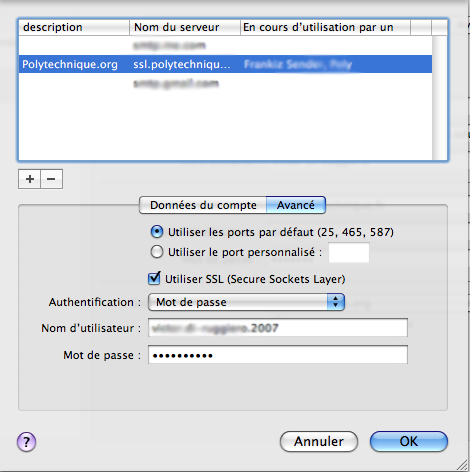
\includegraphics[width=0.4\textwidth]{images/mac_config_smtp_poltechnique.png}
%      \caption{Configurer le serveur SMTP \server{Polytechnique.org}}
%    \end{center}
%  \end{figure*}
%
%%Le LDAP ne fonctionne pas à  l'heure actuelle avec \app{Mail} (mars 2009) sous \app{Leopard}, contrairement aux  autres systèmes d'exploitation (fonctionne cependant avec \app{Thunderbird}).
%%\subsuEnfin, tu peux disposer dans \app{Mail} de l'annuaire de l'àcole, mis à  disposition par la DSI. Pour cela, va dans les \menu{Préférences} de Mail,
%%puis dans la rubrique \menu{Rédaction} et clique sur \menu{Configurer LDAP\ldots}. Tu peux ensuite utiliser le bouton \menu{+} pour ajouter un
%%serveur, et remplir la fenêtre comme sur la capture.
%
%%\imagepos{images/mac_config_ldap}{0.6}{Configurer l'annuaire}{!ht}
%%bsection{Logiciels additionnels}
%
%%Les logiciels suivants sont utiles pour utiliser avec Mac OS X les services proposés sur le réseau~; ils sont téléchargeables sur \server{frankiz}, dans la rubrique \menu{Télécharger}, \menu{Mac}.



%%%%%%%%%%%%%%%%%%%%%%%%%%%%%%%%%%%%%%%%%%%%%%%%
% ANCIENNE CONFIGURATION DES BR POUR CHAQUE OS %
%%%%%%%%%%%%%%%%%%%%%%%%%%%%%%%%%%%%%%%%%%%%%%%%

%% VIEILLE PAGE DE CONF NEWSGROUP POUR WINDOWS

%\subsubsection{Configuration \emph{newsgroups}}
%
%Reporte-toi a la page~\pageref{newsgroups} pour la description et des détails de fonctionnement des \emph{newsgroups} à  l'X.
%
%Comme pour les \emph{mails}, nous décrivons la configuration de \app{Outlook Express} mais elle est sensiblement équivalente pour \app{Thunderbird}. Lance
%\app{Outlook Express} et va dans le menu \menu{Outils}, \menu{Comptes\ldots}. Clique sur le bouton \menu{Ajouter\ldots} en haut à  droite,
%\menu{News\ldots}. Remplis les écrans de configuration suivants avec ces données~:
%\begin{description}
%  \item[Nom complet] ton nom~!
%  \item[Adresse de messagerie] de la forme \mail{prenom.nom@polytechnique.edu}
%  \item[Serveur de news (NNTP)] \server{news}~; vérifie à  ce moment que la case
%       \menu{Connexion à  mon serveur de news requise} n'est pas cochée.
%\end{description}
%Voilà , clique sur \menu{Continuer}, \menu{Terminer}; tu es abonné
%au serveur \emph{news} des élèves.
%
%Quand tu fermeras la fenêtre `Comptes Internet', il va te demander à
%quels \emph{newsgroups} tu veux t'abonner, tu n'auras qu'à  sélectionner
%ceux qui t'intéressent. Reporte-toi à  la page \pageref{newsgroups}
%pour plus d'infos sur les newsgroups auxquels t'abonner~!
%
%Si tu veux t'inscrire à  d'autres serveurs \emph{news}, refais cette
%procédure en rentrant le nom du serveur qui t'intéresse à  la place
%de \fkz.
%\setcounter{page}{12}

%% VIEILLE PAGE DE CONF NEWSGROUPS POUR LINUX


%\subsubsection{Configuration \emph{news}}
%
%\flimage{images/nux_knode_icon}{0.12}{l} Le client \emph{news} le plus utilisé est \app{Knode}. Parmi les autres clients \emph{news}, citons
%\app{Thunderbird}, \app{Pan} ou \app{slrn}. Ici aussi, la configuration est presque indépendante du logiciel choisi.
%
%
%Sous \app{Knode}, c'est dans le menu \menu{Configuration}, puis \menu{Configurer Knode}. Va dans la rubrique \menu{Comptes, Forums de discussion} et
%crée un compte en cliquant sur \menu{Ajouter\ldots}.
%
%\imagepos{images/nux_config_knode}{0.45}{Configuration de Knode}{ht}
%
%\pagebreak
%
%Remplis l'onglet \menu{Serveur} avec les informations suivantes~:
%\begin{description}
%  \item[Nom] ce que tu veux pour décrire ce compte, par exemple 'News Frankiz'
%  \item[Serveur] \server{news}
%\nopagebreak  \item[Port] 119
%\end{description}
%
%\pagebreak
%
%Ensuite occupe-toi de l'onglet \menu{Identité}~:
%\begin{description}
%  \item[Nom] mets ton pseudo dans ce champ
%  \item[Organisation] X, École polytechnique, comme tu le sens
%  \item[Adresse électronique] ton adresse \emph{mail}, pour que les gens puissent te répondre par \emph{mail}.
%\end{description}
%
%Enfin, pour que \app{Knode} puisse envoyer des \emph{mails}, il faut aller
%dans la rubrique \menu{Comptes}, sous-rubrique \menu{Serveur de
%courrier (SMTP)}, et choisir comme serveur d'envoi de \emph{mails}
%\server{poly.polytechnique.fr}, port 25 --- c'est exactement la même
%configuration SMTP que \app{Kmail}.
%
%Si tu veux mettre une signature à  la fin des messages que tu
%posteras, il te suffit de la mettre dans l'onglet \menu{Identité}.
%Sur la plupart des clients la signature est interprétée comme
%extérieure au message et n'est en particulier pas incluse dans le
%texte cité lorsque tu réponds à  un message. Pour définir une
%signature à  la main, il suffit de mettre \verb*+-- +\ (c'est à  dire
%-{}-<espace>) sur une ligne, et tout ce qui suivra cette ligne
%composera ta signature.
%
%Il ne te reste plus qu'à  t'inscrire à  des \emph{newsgroups} (reporte-toi à  la page \pageref{newsgroups} pour plus d'infos) et à  poster~! \\
%
%Pour te connecter aux serveurs de \emph{news} de Polytechnique.org, qui ont un accès sécurisé, avec \app{Knode}, il y a une petite subtilité car il
%ne gère pas le SSL. Il faut installer \app{stunnel} qui permet de définir une redirection SSL de port. Dans \file{/etc/stunnel.conf} (ou parfois \file{/etc/stunnel/stunnel.conf}), mets les lignes suivantes (les trois premières y sont en principe déjà )~:
%\cmdline{\# location of pid file\\
%pid = /etc/stunnel/stunnel.pid\\
%\\
%\# user to run as\\
%setuid = stunnel\\
%setgid = stunnel\\
%\\
%\# Use it for client mode\\
%client = yes\\
%\\
%\# sample service-level configuration\\
%{[}nntps{]}\\
%accept  = 1119\\
%connect = ssl.polytechnique.org:563\\
%TIMEOUTclose = 0
%}
%
%Il ne te reste plus qu'à  lancer \app{stunnel} par~:
%\cmdline{/etc/init.d/stunnel start}
%
%Et tu peux ainsi lire les \emph{news} de Polytechnique.org en mettant \server{localhost} comme serveur et
%\server{1119} comme port. Il faut aussi que tu coches \menu{Le serveur exige une identification} et
%que tu rentres ton nom d'utilisateur à  Polytechnique.org et ton mot de passe, que tu peux définir
%sur \urllink{https://www.polytechnique.org/Xorg/SMTPSecurise}.

%% VIEILLE PAGE DE CONF NEWSGROUP POUR MAC


%\subsubsection{Configuration \emph{news}}
%
%\flimage{images/mac_thunderbird_icone}{0.07}{l}
%\app{Thunderbird}~: un client \emph{news} permettant d'accéder aux forums de discussion des élèves (voir page~\pageref{newsgroups} pour les détails sur \server{frankiz}), mais aussi à  ceux de \server{usenet} grâce au serveur \server{polynews.polytechnique.fr}. Il est très proche d'\app{Outlook Express} dans son esprit. Dans la même catégorie, il existe \app{MacSOUP}, \app{Unison} ou encore \app{MT-NewsWatcher}. La configuration se fait de la même manière.
%
%Au premier lancement, l'application te propose d'importer les paramètres depuis une autre application. Clique sur \menu{Suivant}. Tu peux alors choisir quel type de compte tu veux configurer (tu remarqueras que tu peux aussi créer un compte courrier électronique, et un compte RSS). Sélectionne \menu{Compte forums de discussion} et clique sur \menu{Suivant}. Entre alors les informations suivantes~:
%
%\begin{description}
%  \item[Votre nom] ton nom ou ton pseudo
%  \item[Adresse de courrier] \mail{prenom.nom@polytechnique.edu}
%  \item[Serveur de forums] \server{news}
%  \item[Nom du compte] News Frankiz
%  \item[Nom d'utilisateur] ton \emph{login }poly (les huit premières lettres de ton nom en général)
%  \item[Serveur d'envoi (SMTP)] \server{poly.polytechnique.fr} ou \server{ssl.polytechnique.org}
%\end{description}
%
%
%Pour t'abonner à  des groupes de discussion, il te suffit de sélectionner le compte \menu{News Frankiz} dans la fenêtre \menu{Dossiers} de \app{Thunderbird}, puis de cliquer sur \menu{Gérer les abonnements aux groupes de discussion}. Tu pourras ensuite sélectionner les forums qui t'intéressent parmi la liste proposée. Reporte-toi à  la page \pageref{newsgroups} pour plus d'infos sur les \emph{newsgroups} auxquels t'abonner~!
%
